\chapter{Umsetzung}

Die Sensoren werden an einen Raspberry Pi angeschlossen und melden die
gemessenen Werte an einen zentralen Raspberry Pi. Der zentrale Raspberry Pi legt
die gemeldeten Daten in einer Datenbank ab. Eine Webseite greift auf die
Datenbank zu und stellt die Daten dar.\\
Die Kommunikation wird über ein eigenes WLAN-Netz abgewickelt das von der
Zentraleinheit aufgespannt wird. IP-Adressen werden von einem \ac{DHCP}-Server, der
auf der Zentraleinheit installiert ist vergeben.\\
Die Website wird durch einen Apache-Webserver auf der Zentraleinheit
bereitgestellt.
%
%%
%Harm
\section{Netzwerkkonfiguration}
%TODO: Einleitender satz
%TODO: WLAN-Stick
%TODO: Acro WLAN Anmerkung: WLAN ist eine allgemein bekannte Abkürzung und muss nicht erklärt werden!!
%Passt
\subsection{WLAN}
%TODO: Wird von der Zentraleinheit aufgespannt
Es wird ein Funknetz auf Basis des 802.11n Standards verwendet. Aufgespannt wird das WLAN von der Zentraleinheit, auf der zentrale Dienste bereitgestellt werden. Als Name wurde Pinet festgelegt, der von allen gesehen werden kann. In der Tabelle (siehe \fullref{tab:WLAN-Konfiguration}) sind die einzelnen Optionen aufgeführt und erläutert.

 
\begin{table}
\caption{WLAN-Konfigurationsdetails}
\label{tab:WLAN-Konfiguration}
\begin{tabular}{p{0.5\textwidth} p{0.45\textwidth}}
\textbf{Befehl} 						& \textbf{Erklärung} \\
interface=wlan0 						& Das Interface auf dem das Funknetz ausgestrahlt wird \\
ssid=Pinet 									& Der Name des Funknetzes \\
country\_code=DE 						& Über die Festlegung der Region wird sichergestellt, dass das Funknetz die spezifischen Grenzwerte für Kanäle oder Sendestärke einhält \\
hw\_mode=g 									& Legt fest, dass das Funknetz im 2,4 GHz-Band ausgestrahlt wird \\
channel=6 									& Der Funkkanal 6 wird verwendet \\
macaddr\_acl=0 							& MAC-Adressenfilterung ist deaktiviert \\
auth\_algs=1 								& Legt fest, dass als Verschlüsselung \ac{WPA} verwendet wird \\
ignore\_broadcast\_ssid=0 	& Die \ac{SSID} wird ausgestrahlt und nicht versteckt. \\
wpa=2 											& Legt die WPA-Version fest auf \ac{WPA2} \\
wpa\_passphrase=********** 	& Legt den \ac{PSK} fest \\
wpa\_key\_mgmt=WPA-PSK 			& Legt fest, dass ein \ac{PSK} verwendet wird \\
wpa\_pairwise=CCMP 					& Legt fest, dass nur der \ac{AES}-Verschlüsselungsalgorithmus verwendet wird \\
wpa\_group\_rekey=86400 		& Legt fest, dass alle 86400 Sekunden ein neuer Schlüssel verwendet werden muss \\
ieee80211n=1 								& Aktiviert den n-Standard \\
wme\_enabled=1 							& Aktiviert \ac{QoS} - Voraussetzung für die Verwendung des n-Standards \\
 \end{tabular}
\end{table}
%passt
\subsection{Verschlüsselung}

Wie aus der \fullref{tab:WLAN-Konfiguration} hervorgeht, ist das WLAN mit \ac{WPA2} verschlüsselt. \ac{WPA2} gilt aktuell als sicher, was nicht für die Alternativen \ac{WEP} oder \ac{WPA} gilt. Zur Authentifizierung wird ein \ac{PSK} verwendet. Als Verschlüsselungsprotokoll wird \ac{CCMP} verwendet. 

%passt
\subsection{\ac{DHCP}}
 
Als \ac{DHCP}-Server wird der ISC-DHCP-Server verwendet.\\
Die IP-Adressen werden nur über das wlan0-Interface der Zentraleinheit vergeben. Als Netz wird das private Netz 192.168.178.0 /24 verwendet. In diesem Netz hat die Zentraleinheit als \ac{DHCP}-Server die Adresse 192.168.178.1 /24. Diese Adresse ist statisch eingetragen. Alle anderen Geräte erhalten dynamische IP-Adressen aus dem Bereich 192.168.178.10 - 192.168.178.250. Die Lease-Time wurde auf 604800 Sekunden festgelegt. Dies entspricht 7 Tagen. Als Lease-Time wird der Zeitraum bezeichnet, in dem ein Netzwerkgerät, die gleiche IP-Adresse erhält. So wird verhindert, dass viele Adressänderungen stattfinden. Da nur wenige Geräte im Netz verfügbar sind und auch keine häufigen Änderungen erwartet werden, wird der Zeitraum von 7 Tagen als ausreichend angesehen. Damit der \ac{DHCP}-Server die IP-Adressen nur im WLAN vergibt, wird die IP-Adress-Vergabe auf das Interface wlan0 eingeschränkt.



\begin{lstlisting}[caption=Konfiguration des ISC-DHCP-Server,frame=single,label=dhcpkonfig]
#Rogue-DHCP-Server nicht erlauben (Doppelter DHCP-Server)
authoritative;

#Definition des Subnetzes
subnet 192.168.178.0 netmask 255.255.255.0
{
        #Angabe der DHCP-Range
        range 192.168.178.10 192.168.178.250;

        #Angabe der Lease-Times 7 Tage in sekunden
        default-lease-time 604800;
        max-lease-time 604800;

        #Begrenzung auf das WLAN-Interface
        interface wlan0;
}

\end{lstlisting}

%Alex
%Passt
\section{Sensorknoten} %Allgemein Vorinstalation!
Für die Umsetzung des Sensorknotens werden vorab Pythonbibliotheken benötigt. Sie werden mit dem folgenden Befehl im Quellcode hinzugefügt:
\begin{lstlisting}[caption=Importbefehl in Python,frame=single,numbers=left,language=Python]
# Hinzufügen eines kompletten Paketes
import <Paketname> as <Aliasname>
# Hinzufügen einer Methode aus einem Paket
from <Paketname> import <Methodenname>
\end{lstlisting}
%TODO: Tabelle daraus machen
Folgende Pakete werden benötigt:
\begin{enumerate}
	\item RPi.GPIO
	\item smbus
	\item socket
	\item json
	\item Adafruit\_DHT
\end{enumerate}

RPi.GPIO ist die Bibliothek zur Nutzung der \ac{GPIO} Schnittstelle in Python. Das Paket smbus ermöglicht den Zugriff auf die I$^2$C Schnittstelle. Das Paket socket ermöglicht die Nutzung der TCP/IP Socketverbindung. Mittels json kann das Datenformat \ac{JSON} genutzt werden. Python bietet mit Hilfe der Adafruit\cite{Adafruit60:online} Bibliotheken eine Schnittstelle zu den Sensoren. Die Adafruitbibliothek kann mit Hilfe des pythoneigenen Paketmanagers, "'pip"', installiert werden.
\begin{lstlisting}[caption=Installation der Adafruit Bibliothek mit pip,frame=single]
pip install adafruit_python_dht
\end{lstlisting}
Dieses Paket wird zum Ansteuern des DHT-11 Sensors, der im \fullref{Sensoren_Planung} beschrieben wird, benötigt. Die genutzte Erweiterungsplatine RPI - Explorer 700 benötigt keine zusätzliche Software. Die Platine muss auf die \ac{GPIO} Pins gesteckt werden, um funktional zu sein. Der \ac{A/D-Wandler} befindet sich neben den \ac{GPIO} Anschlüssen und hat eine gelbe Platinenfarbe. Bevor der \ac{A/D-Wandler} einsatzfähig ist muss der I$^2$C Bus in der Raspi-config Datei aktiviert werden. Mit dem aktiven I$^2$C Bus können die Sensoren ausgelesen werden.
%Passt
\subsection{Verdrahtung der Sensoren}\label{Verdrahtung_der_Sensoren}
%Die Sensoren werden bestimmten Pins zugewiesen, damit sowohl erfahrene als auch unerfahrene Nutzer dieses Sensorknotensystem nachbauen können.
Die Sensoren, aus dem \fullref{Sensoren_Planung}, haben eine feste Zuweisung an die jeweiligen Pins. Dies ermöglicht es anderen Nutzern das System einfacher und schneller nachzubauen, ohne Probleme bei der Verbindung der Sensoren zu bekommen. Die Tabelle \fullref{tab:Pinbelegung} beschreibt die Belegung der einzelnen Pins.
\begin{table}[htp]
	\caption{GPIO und analoge Pinbelegung der Sensoren}
	\label{tab:Pinbelegung}
	\begin{tabular}{p{0.15\textwidth} p{0.2\textwidth} p{0.6\textwidth}}
		\textbf{GPIO-Pin}	& \textbf{Sensor} & \textbf{Beschreibung} \\
		Pin 5 		& Schocksensor 	& Funktionsweise über die Flankendetektion\\	
		Pin 17		& Flammensensor	& True oder False Wert vom Sensor\\
		Pin 18		& Mikrofon		& True oder False Wert vom Sensor\\
		Pin 24		& Lichtschranke	& True oder False Wert vom Sensor\\
		Pin 25		& DHT11 Sensor	& Luftfeuchtigkeits- und Temperaturwerte werden als digitale Werte geliefert
	\end{tabular}
\end{table}
\begin{table}[htp]
	\begin{tabular}{p{0.15\textwidth} p{0.2\textwidth} p{0.6\textwidth}}
		\textbf{Analog-Pin}	& \textbf{Sensor} & \textbf{Beschreibung} \\
		A0	& Mikrofon 		& Analoge Messwerte des Mikrofons. Werden zur Fehlererkennung genutzt. \\
		A1	& Flammensensor	& Analoge Messwerte des Flammensensors. Werden zur Fehlererkennung genutzt.\\
		A2	& Lichtsensor	& Analoge Messwerte des Lichtsensors.
	\end{tabular}
\end{table}

 Der zusätzliche analoge Ausgang des Flammensensors und des Mikrofons wird zur Messwertüberprüfung genutzt. Als einziger Sensor der Lichtsensor besitzt keine direkte Anschlussmöglichkeit an einen \ac{GPIO} Pin und kann somit nicht zusätzlich auf Messfehler untersucht werden. Der Aufbau der \ac{GPIO} Steckplatine beeinflusst zusätzlich die Pinbelegung der Sensoren. Wie in \fullref{fig:Kapitel2/gpio_pins_pi2.png} zu sehen ist, sind die Pins 9, 14, 20 und 25 Masseanschlüsse. Die genutzten Sensoren befinden sich in unmittelbarer Nähe zu diesen. Zum einen können sich Nutzer an den Positionen der Masseanschlüsse orientieren und zum anderen ebenfalls schneller den korrekten Pin finden. Ein weiterer Vorteil ist, dass im Falle eines versehentlichen Fehlanschließens keine Gefahr für den Sensor entsteht, da beispielsweise auf den digitalen Ausgangspin keine 5V Eingangsspannung gelangen kann. Durch die feste Pinbelegung entsteht eine feste Vorgabe der Anschlussarchitektur. Die Sensoren können falsch angeschlossen werden und würden dabei ebenfalls Messdaten erzeugen, doch eine korrekte Zuweisung der Messdaten an die Sensoren wäre nicht möglich. Des Weiteren hat die feste Pinbelegung ebenso einen Einfluss auf die Implementierung der Sensoren. 
\subsection{Implementierung der Sensoren}\label{Sensorknoten:Implementierung}
% Lichtsensor: Problematisch ist hierbei das Tageslicht, da es das gleiche Verhalten beim Sensor auslöst.
% Schocksensor:Eine Umsetzung mit diesem Modell ist nicht mögich, da eine starke Erschütterung zum detektieren benötigt.
Bevor die Sensoren implementiert werden können, muss eine Softwarearchitektur aufgebaut werden. Zuerst gibt es die Auswahl eines objektorientierten oder nicht objektorientierten Ansatzes.
Ein Vorteil der \ac{OOP} ist die Erweiterungsfähigkeit. Eine neue Funktion kann in der Klasse niedergeschrieben werden und zur Laufzeit ausgeführt werden. Des Weiteren können mehrere Instanzen einer Klasse zur Laufzeit erzeugt werden. Somit kann eine Hauptklasse erstellt werden, die dann zur Laufzeit mehrere Objekte erzeugen kann, die jeweils eine eigene Funktionalität ausüben. Eine weitere Problemstellung in der Entwicklung der Softwarearchitektur ist die Klassenhierarchie. Statt den gewöhnlichen Ansatz einer Hauptklasse und dann jeweils einer Unterklasse mit einer Funktionalität auszubauen, wird hierbei der Ansatz einer monolithischen Architektur gewählt. Im Sensorknoten werden nur Sensoren implementiert. Damit würde es eine Überklasse geben, wovon jeder Sensor erben würde. Beim monolithischen Ansatz gibt es nur eine Klasse, die alle Methoden enthält. Erst bei der Initialisierung kann entschieden werden, welche Funktion ausgeführt werden soll. Eine Instanz einer monolithischen Klasse kann somit, falls es einen Anlass dafür gibt, unabhängig von der Initialisierung ihre Funktionsweise wechseln. Beim klassischen objektorientierten Ansatz müsse eine komplett neue Instanz erzeugt werden. Ein Nachteil der monolithischen Architektur ist die Anhäufung von Methoden in einer Klasse. Ab einem gewissen Grad wird die Klasse schwer wartbar, da zu viele Methoden kontrolliert werden müssen. Diese Größe der Klasse kann weitere Fehler, wie das nicht korrekte Bereinigen von Bugs mit sich bringen. Das größte Problem dieser Architektur ist die fehlerhafte Instanziierung eines Objektes. Zur Darstellung des Problems dient folgendes Programmbeispiel:

\begin{lstlisting}[caption=Fehlerhafte Instanziierung eines Sensorobjektes,frame=single,numbers=left,language=Python, showstringspaces=false]
# Initialisierung des Mikrofons
 sensor1 = Sensor(5, A0, 18)
# Korrekte Ausführung des Mikrofonsensors
<@ \textcolor{green}{\Checkmark} @> sensor1.mikrofon()
# Versuchte Ausführung der der Flammensensor Funktion mit dem Mikrofonobjekt
<@ \textcolor{red}{\XSolid} @> sensor1.flammensensor() 
\end{lstlisting}
Wie in Zeile 2 zu sehen ist, wird ein Sensorobjekt, mit der Bezeichnung "'sensor1"', mit 3 Eingabeparametern initialisiert. Diese werden im späteren Verlauf weiter erläutert. Sensor1 kann jetzt jede Methode der Sensorklasse ausführen. Dei der Initialisierung wurden die festen Angaben eines Mikrofonsensors angegeben. Damit ist die Zeile 4 die einzig korrekte Ausführung für dieses Sensorobjekt. Die Fehlerprüfung durch den Compiler wird bei dieser Architektur nicht unterstützt. Wie in Zeile 6 zu sehen ist, kann die Flammensensorfunktion aufgerufen werden. Für den Compiler ist es ein korrekter Aufruf der Flammensensormethode, jedoch würde diese lediglich fehlerhafte Messdaten zurückgeben. Die Funktionsweise der Sensorklasse wir in den folgenden Schritten erläutert.

\subsubsection*{Der Konstruktor} \label{Methode:Konstruktor}
	Wie in anderen Programmiersprachen, wird ebenfalls in Python ein Konstruktor für das Objekt benötigt. Der Konstruktor initialisiert alle notwendigen Variablen für das Objekt der Klasse. Im Falle des Sensorknotens sieht der Konstruktor wie folgt aus:
		\lstinputlisting[label={LST:Konstruktor},caption=Konstruktor der Sensorklasse,frame=single,numbers=left,language=Python, firstline=10, lastline=26]{Quellcode/sensor.py}

	\textsc{Eric Matthes} beschreibt in seinem Buch "Python crash course"\cite{1593276036} die Funktion \_\_init\_\_ als eine geschützte Funktionalität von Python. Der Zweck der doppelten Unterstriche seie die Abgrenzung von möglichen Namen, die ein Programmierer vergeben dürfe. Es ist üblich, dass einfache Unterstriche zum verbinden von mehreren Wörtern genutzt werden. Somit, weiß der Programmierer, dass diese besondere Funktion nicht anders verwendet werden darf. Eine weitere Auffälligkeit ist die 'self' Variable. Nach \textsc{Eric Matthes} müsse der Parameter an erster Stelle im Konstruktor stehen. Dieser seie für den Bezug auf das Objekt relevant. Das 'self' ist in der Funktionalität ähnlich wie das 'this' aus Java. Die weiteren Übergabeparameter haben folgende Bedeutung:
	\begin{description}
		\item[SEN\_ID] \hfill \\
			Die SEN\_ID ist die feste Nummer des Sensors. Die Nummerierung entstammt dem \fullref{Sensoren_Planung}. Hierbei hat der Temperatursensor die Nummer 1 und der Luftfeuchtigkeitssensor die Nummer 2. Die restlichen Sensoren werden entsprechend hochgezählt. Die SEN\_ID wird für die Zuordnung des Messwertes zum Sensor in der Datenbank benötigt. 
		\item[Analog\_PIN] \hfill \\
			Der Analog\_PIN Übergabeparameter wird für das Ansprechen des A/D-Wanderls benötigt. Die Angaben können aus der \fullref{tab:Pinbelegung} entnommen werden.
		\item[Digital\_PIN] \hfill \\
			Die Nummerierung der Digital\_Pins kann ebenfalls aus der \fullref{tab:Pinbelegung} gelesen werden. Die Angabe wird für Sicherheitsüberprüfungen und zum Auslesen von den digitalen Sensorwerten benutzt.
   	\end{description}
	Der Sensorname ermittelt mit Hilfe der "'socket"' Bibliothek den Namen des Betriebssystems. Damit wird der Name des Sensorknotens ermittelt. Dieser wird für die Zuweisung der Sensoren zum Sensorknoten in der Datenbank genutzt. Der eigentliche Name des jeweiligen Sensors ist für den Sensorknoten nicht von Bedeutung, denn die SEN\_ID ist immer eindeutig. Der Name des Sensors wird mit Hilfe der Datenbank bestimmt.
	%TODO: Verknüpfung zur Zentraleinheit : Datenbank. Übersetzung SEN_ID zum Sensornamen
	Neben der SEN\_ID ist der Messwert in der zu übertragenden Nachricht an die Zentraleinheit enthalten. Der Messwert wird zu Beginn als ein leerer String vorgeladen. Python setzt keine Deklaration vor der Nutzung einer Variable voraus. Die Messwertvariable wird dennoch deklariert, damit der Quellcode wartbarer wird. Die Status Variable dient als Zustandskontrolle des Sensors. Der Status des Sensors wird auf der Webseite wie im Kapitel BLAARRRGH %TODO: Verweis auf Website Übersicht mit dem Statusbit!
	erläutert, dargestellt. Der Zustand ändert sich explizit, sobald ein Sensor detektiert wird. Die Status-Variable kann folgende Zustände annehmen:
	\begin{description}
		\item[Status = 0] \hfill \\
			Bedeutet, dass der Sensor nicht angeschlossen ist. Dies ist außerdem der Defaultzustand aller Sensorobjekte.
		\item[Status = 1] \hfill \\
			Bedeutet, dass der Sensor angeschlossen ist. Dieser Zustand soll dem Benutzer signalisieren, dass der Sensor korrekt arbeitet.
		\item[Status = 2] \hfill \\
			Bedeutet, dass der Sensor defekt ist. Anders als beim Zustand 0 tritt dieser Fall erst auf, wenn ein unmöglicher Messwert gemessen wurde. Ein Beispiel hierfür ist: Falls der Temperatursensor, welcher einen Messbereich von 0 bis 50$^\circ$C hat, Messwerte unter dem Gefrierpunkt oder über 50$^\circ$C liefert.
	\end{description}
	Die Zeile neun im \fullref{LST:Konstruktor} dient zur Einstellung der GPIO-Pinbezeichnung. \textsc{MATT} beschreibt in seinem Blogeintrag "'Simple Guide to the RPi Header and Pins'"\cite{SimpleGu6:online}, dass es zwei mögliche Modi für diesen Befehl gebe. Zum einen gibt es den Übergabeparameter "'GPIO.BOARD"' und zum anderen "'GPIO.BCM"'. Sie würden für die verschiedenen Nummerierungsmöglichkeiten der \ac{GPIO} Schnittstelle stehen. GPIO.BOARD würde die Nummerierung der Pins nach der Position auf dem Board durchführen. Im Gegensatz dazu nutze die GPIO.BCM Nummerierung die eigentliche GPIO Pinbelegung. Diese wir in der \fullref{fig:Kapitel2/gpio_pins_pi2.png} dargestellt.\\
	Die Ausgabe von Warnungen der GPIO Bibliothek wird mit dem Befehl in der zehnten Zeile deaktiviert. Diese sind nicht notwendig, da zum einen die Sensorenknoten an keiner graphischen Ausgabe angeschlossen sind und zum anderen Fehler separat behandelt werden.\\
	Falls der Sensor einen digitalen Anschluss hat, muss dieser initialisiert werden. Dazu dient die Kontrollstruktur von Zeile elf bis vierzehn. \textsc{Chris Hager} beschreibt in der "RPIO 0.10.0 documentation - RPIO, the Python module" den Befehl "GPIO.setup()"\space wie folgt: Der Befehl benötige als Übergabeparameter den Pin, den Modus - entweder GPIO.IN oder GPIO.OUT - die Angabe, ob der Pull-up oder Pull-down Widerstand aktiv sein solle. Im Falle der Sensoren muss das Signal als "GPIO.IN" deklariert werden. Es wird weder ein Pull-up noch ein Pull-down Widerstand angeschlossen. Aus diesem Grund wird als letzter Parameter "'GPIO.PUD\_OFF"' angegeben. \\
	Die letzten zwei Befehle dienen zum Initialisieren des I$^2$C Buses. Der '"smbus.SMBus(X)"' nimmt entweder den Wert 0 oder Wert 1 an. Nach einem empirischen Test hat es sich herausgestellt, dass die Raspberry Pis in der Version 2 und 3 das i2c-dev1 Interface standardmäßig nutzten. Somit muss der Befehl "'smbus.SMBUS(1)"' ausgeführt werden. Die Adresse des I$^2$C Ports muss ebenfalls angegeben werden. Nach dem Blogeintrag "GPIO Interface library for the Raspberry Pi"\cite{I2CPCF8592:online} von Wiring Pi seie die Adresse "0x46$_H$"\space die Standardadresse des I$^2$C Ports im Raspberry Pi. Damit ist der Konstruktor abgeschlossen und es folgen die Methoden der Sensorklasse.
	
%Hacken
\subsubsection*{Aufräumfunktion}
	Diese Funktion dient zum Aufräumen der \ac{GPIO} Anschlüsse. \textsc{Ben Croston} schreibt in seinem Artikel "'RPi.GPIO basics 3"' \cite{RPiGPIOb90:online}, dass die \ac{GPIO} Pins aufgeräumt werden sollten. Folgendes Problem bestehe beim Raspberry Pi: Falls ein Port im Programm auf den Wert "'1"' gesetzt wurde, behalte dieser den Wert auch nach dem Beenden des Programms. Würde der Nutzer versehentlich den Anschluss mit einem Masseanschluss verbinden, so wäre es möglich, dass die Platte durch einen Kurzschluss Schäden davon trage. Die Implementierung für die Sensorklasse sieht wie folgt aus:
	\lstinputlisting[caption=Portbereinigungsmethode mittels GPIO.cleanup,frame=single,numbers=left,language=Python, firstline=28, lastline=29, showstringspaces=false]{Quellcode/sensor.py}
	Nach \textsc{Ben Croston} \cite{RPiGPIOb90:online} reinige die GPIO.cleanup Funktion nur die verwendeten Ports den jeweiligen Objektes. Somit muss diese Funktion von jeweiligen Sensorobjekten ausgeführt werden. Semantisch gesehen gehört die Funktion in die Sensorklasse, dennoch befindet sie sich eine Abstraktionsstufe über dieser. Die Pins können erst aufgeräumt werden, sobald ein Sensorobjekt nicht mehr gebraucht wird. Somit gehört diese Funktion erst zur Geltung, nachdem das Hauptprogramm	beendet wurde.
\subsubsection*{Bindung der Eventsteuerung des Flammensensors und des Mikrofons}
	Der Flammensensor unterscheidet sich in seinem Verhalten nicht vom Mikrofon. Da beide ein Auslösesignal zur Detektion eines Ereignisses benötigen, werden die Funktionen zusammengefasst dargestellt. Das folgende Listing stellt die Implementierungen der Eventsteuerung dar.
	\lstinputlisting[caption=Hinzufügen der Eventsteuerung für den Flammensensor und das Mikrofon,frame=single,numbers=left,language=Python, firstline=31, lastline=41,showstringspaces=false]{Quellcode/sensor.py}
	Die GPIO Bibliothek bietet mit der Funktion "'add\_event\_detect"' eine Möglichkeit eigene Flankenauslösungen zu implementieren. Der Befehl benötigt die Angabe des digitalen Pins, welche Flanken detektiert werden sollen, den darauffolgenden Methodenaufruf und zum Schluss die Wiederholzeit. Der digitale Pin wird mit der Angabe "'Digital\_Pin"', wie im \fullref{Methode:Konstruktor} angegeben, festgelegt. Die GPIO Bibliothek unterstützt mit dem Parameter "'GPIO.RISING"' die steigende, mit "'GPIO.FALLING"' die fallende und "'GPIO.BOTH"' beide Flanken zu detektieren. Zur Ermittlung eines Ereignisses genügt die steigende Flanke. 
	
	Damit wäre der Ablauf des Programms gefährdet, denn sobald ein Ereignis festgestellt wurde, wäre das Programm nicht in der Lage diesen gesetzten Zustand zu verlassen. Deshalb werden beide Flanken betrachtet. Die fallende Flanke löst das Zurücksetzen des Flags aus und zeigt damit dem Benutzer, dass das Ereignis beendet wurde. Ohne die fallende Flanke wäre die einzige Möglichkeit des Zurücksetzens ein Neustart des Programms. 
	
	Die Angabe des "'callbacks"' legt die auszuführende Funktion bei einer Flankendetektion fest. Der letzte Parameter ist eine Analogie zum Prellverhalten von mechanischen Tastern. Damit kann eine Sperre in Millisekunden angegeben werden. Dies soll eine Dopplung des Signals verhindern.
\subsubsection*{Eventsteuerung des Flammensensors und des Mikrofons}
	Nachdem die Vorbedingungen für die Eventsteuerung gelegt sind, kann die eigentliche Implementierung fortgeführt werden. Folgender Programmausschnitt verdeutlicht diese:
	\lstinputlisting[caption=Implementierung Eventsteuerung des Flammensensors und des Mikrofons,frame=single,numbers=left,language=Python, firstline=52, lastline=81]{Quellcode/sensor.py}
	Die erste Auffälligkeit dieser Methode ist der "'null"' Übergabeparameter. Dieser hat seinen Ursprung in der callback Funktion des vorherigen Unterthemas. Der callback Funktionsaufruf übergibt immer einen Wert an seine Funktion. In diesem Fall wird kein Übergabeparameter vorausgesetzt, da die Funktion die Berechnungen durchführen soll. 
	
	Die im \fullref{Methode:Konstruktor} beschriebene Statusvariable wird, beim Eintritt in die Funktion auf den Wert "'Angeschlossen"' gesetzt. Diese Funktion wird nur aufgerufen, wenn eine Flanke detektiert wurde. Somit muss der Sensor erstmals als funktional angesehen werden. Ob der Sensor fehlerfrei arbeitet, wird im späteren Verlauf festgestellt. Bevor das analoge Signal ausgelesen werden kann, muss der \ac{A/D-Wandler} angesprochen werden. Der Befehl in der dritten Zeile schreibt die Werte des Busses an der $I^2C$ Adresse an den eingestellten analogen Pin. Im nächsten Schritt wird der gemessene analoge Wert in der Variable "'Analog\_Wert"' abgespeichert. 
	
	Der digitale Wert wird mittels "'GPIO.input"' eingelesen. Mit diesem wird ermittelt, ob es sich um eine steigende oder um eine fallende Flanke handelt. Abhängig von dieser Flanke wird entweder ein positiver oder ein negativer Wert an die Zentraleinheit versendet. Falls der digitale Wert "'1"' ist, handelt es sich bei der vorliegenden Flanke um eine steigende Flanke. 

	Durch empirische Untersuchungen wurde festgestellt, dass der Flammensensor und das Mikrofon bei einem Defekt einen Wert von "'255"' liefern. Der Wert entspricht einem Kurzschluss des Sensors. Nachdem sichergestellt wurde, dass der Sensor korrekt arbeitet, werden die Daten für die Zentraleinheit vorbereitet. Die notwendigen Daten werden in Form eines \ac{JSON} Objekts versendet. Bei einer korrekten Messung liegt der Messwert "'TRUE"', bei einer nicht erfolgreichen Messung "'FALSE"' und bei einem Defekt der Messwert "'0"' vor. Die unterschiedlichen Werte lösen verschiedene visuelle Darstellungen auf der Webseite aus. Dazu mehr im \fullref{Webseite} mehr.
	
\subsubsection*{Sensorüberprüfung} \label{Sensorueberpruefung}
	In dieser Funktion wird überprüft, ob der angeschlossene analoge Sensor korrekt arbeitet. Durch empirische Untersuchungen wurde festgestellt, dass der vorliegende \ac{A/D-Wandler} bei einem nicht angeschlossenen analogen Sensor einen Messwert von "'0"' angibt. Diese Information wird für die weitere Überprüfung genutzt. Die Umsetzung sieht wie folgt aus:
	\lstinputlisting[caption=Überprüfung ob analoger Sensor angeschlossen ist,frame=single,numbers=left,language=Python, firstline=83, lastline=91]{Quellcode/sensor.py}
	Python liefert im Falle eines nicht initialisierten \acp{A/D-Wandler} einen "'IOError"' Fehler, der auf ein nicht angeschlossenes Eingabe- oder Ausgabegerät hinweist. Der Fehler wird abgefangen und stattdessen wird der Wert "'False"' übergeben. Dieser symbolisiert, dass kein analoger Sensor angeschlossen ist. Wie zuvor erwähnt gibt der \ac{A/D-Wandler} den Wert "'0"' als Referenz auf einen nicht angeschlossenen Eingang zurück. Die hierbei vorliegenden analogen Sensoren haben, sobald sie angeschlossen sind, einen niedrigen Betriebspegel, der im Leerlauf im Bereich 5 - 10 liegt. Falls der Pegel größer als 0 ist, wird angenommen, dass der Sensor angeschlossen ist. Ansonsten wird angenommen, dass kein analoger Sensor angeschlossen ist.
\subsubsection*{Der Flammensensor und das Mikrofon}
	Da sowohl das Mikrofon als auch der Flammensensor gleich aufgebaut sind, ist die Funktionalität des Flammensensors gleich der des Mikrofons. Der Unterschied besteht darin, dass es sich beim Flammensensor um einen optischen Sensor und beim Mikrofonsensor um ein Mikrofon handelt. Daher ist eine Erläuterung des Flammensensors ausreichend für das Verständnis beider Sensoren. Diese unterscheiden sich nur am Aufrufnamen, statt \textit{flammensensor()} wird \textit{mikrofon()} genutzt. Die folgende Erklärung bezieht sich auf den Quellcode des Flammensensors, dient aber ebenfalls für das Verständnis des Mikrofons. Beim Flammensensor werden die Messwerte des analogen Sensors ausgewertet und gegebenenfalls an die Zentraleinheit verschickt. Die Implementierung sieht wie folgt aus:
	\lstinputlisting[caption=Funktionsweise des Flammensensors,frame=single,numbers=left,language=Python, firstline=92, lastline=127]{Quellcode/sensor.py}
	Zu Beginn wird überprüft, ob der Sensor angeschlossen ist. 
	
	Die Funktion "'sensorcheck\_analog()"', die im vorherigen \fullref{Sensorueberpruefung} erläutert wird, entscheidet, welches Paket an die Zentrale geschickt wird. Beim nicht angeschlossenem Sensor werden die Werte Status und Messwert auf "'0"' gesetzt, in ein Paket gepackt und abgeschickt. 
	
	Falls ein Flammensensor angeschlossen ist, wird eine weitere Unterteilung durchgeführt. Der digitale Pin wird auf eine logische "'1"' überprüft mit der Bedingung, dass der analoge Messwert "'Analog\_Wert"' unter 255 sein sollte. 
	
	Durch empirische Untersuchungen wurde festgestellt, dass der Flammensensor selbst bei maximaler Flammendetektion nicht den Messwert "'255"' beim A/D-Wandler erreicht. Somit eignet sich dieser Wert für die Kontrolle der korrekten Funktionsweise des Flammensensors. Falls in Zeile acht die Bedingungen erfüllt sind, muss der Flammensensor eine Flamme registrieren. Dazu wird der Messwert auf "'TRUE"' gesetzt und mit der senden Methode an die Zentrale verschickt. Die senden Methode wird im späteren Verlauf erläutert. Falls der Flammensensor defekt und damit die Zeile 16 gültig ist, wird der Status auf "'2"', der Messwert auf "'0"' gesetzt und ebenfalls an die Zentraleinheit abgeschickt. Falls keine Flamme am Flammensensor detektiert wird, besteht kein Bedarf eine Nachricht an den Server zu schicken. Der Server initialisiert die Webseite mit den Messwert "'FALSE"' für den Flammensensor.
	%Hacken
\subsubsection*{Temperatur- und Luftfeuchtigkeitssensor}
	Der DHT11 Sensor liefert mit der Adafruit Bibliothek beide Messwerte gemeinsam aus. Aufgrund der Programmarchitektur - ein Objekt soll nur eine Funktion haben - wird die Funktionalität in zwei Methoden aufgeteilt. Aufgrund der hohen Ähnlichkeit der beiden Arbeitsweisen werden diese gemeinsam in einem Abschnitt erläutert. Der DHT11 Sensor ist einer der beiden Sensoren, der ohne analoge Signale arbeitet. Damit wird ebenfalls die Kontrollmöglichkeit des Sensors eingeschränkt. Die Implementierung des Temperatursensors ist wie folgt:
	\lstinputlisting[caption=Implementierung der Temperaturfühlerfunktion des DHT11 Sensors,frame=single,numbers=left,language=Python, firstline=129, lastline=148]{Quellcode/sensor.py}
	Die Adafruit\_DHT Bibliothek liefert mit der Funktion "'read.retry()"' eine Möglichkeit den DHT11 Sensor auszulesen. Der erste Übergabeparameter für diese Funktion ist der Modulname des Sensors. Hierbei können laut der Dokumentation der Adafruit DHT Bibliothek\cite{Adafruit47:online} "'11"', entsprechend dem DHT11, "'22"', entsprechend dem DHT22 und "'2302"', entsprechend dem AM2302 Sensor, angegeben werden. Nach der Angabe des Moduls folgt die Eingabe des verwendeten digitalen Pins. Die Funktion liefert als Rückgabewert ein Array mit zwei Speicherstellen. An der Stelle 0 wird die Luftfeuchtigkeit und an der Position 1 die Temperatur gespeichert. Dies hat zur Folge, dass in Zeile zwei die Position "'1"' der Funktionsrückgabe gespeichert wird.
	 %TODO: Grad Zeichen hier korrigieren!
	Der digitale Sensor hat keine Möglichkeit eine unabhängige Fehlerüberprüfung zu gewährleisten. Daher wird zur Fehlerabhandlung der Messbereich des Sensors als Richtwert genommen. Falls die gemessene Temperatur außerhalb eines festgelegten Bereiches liegt, wird angenommen, dass der Sensor defekt sein muss. Hier ist die einzige Unterscheidung zwischen der Temperaturmethode und der Luftfeuchtigkeitsmethode. Bei der Temperatur wird der Bereich 0 bis kleiner gleich 50$\circ$C , während die Luftfeuchtigkeit zwischen 0 und kleiner gleich 95\% gemessen werden kann. Sollte sich der Messwert im messbaren Bereich befinden, wird der Status auf eine "'1"' und der Messwert auf den gemessenen Wert gesetzt. Der Messwert muss jedoch zuvor vom Float-Datentyp in einen Text konvertiert werden, damit es keine Darstellungsprobleme auf der Webseite gibt. Falls kein DHT11 Sensor angeschlossen ist, wird die Funktion in Zeile zwei kein Objekt "'temperatur"' erzeugen. Python besitzt die Fähigkeit auf nicht vorhandene Objekte in einer Kontrollstruktur zu prüfen. Damit wird die Zeile acht im Falle eines nicht vorhandenen Sensors erfüllt und die des Status und des Messwerts auf "'0"' gesetzt. Der else Pfad in Zeile elf wird im Falle eines defekten Sensors ausgeführt. Bei einer Fehlfunktion würde entweder eine "'0"' oder ein sehr hoher Wert gemessen werden. Abschließend werden die Daten mittels der senden Methode an den Server geschickt.
	%Hacken
\subsubsection*{Der Lichtsensor}
	Beim Lichtsensor handelt es sich um einen analogen Photowiderstand, der abhängig von der Helligkeit des Lichts, einen niedrigen oder hohen Widerstand besitzt. Dieser analoge Widerstandswert wird am \ac{A/D-Wandler} in einen digitalen Messwert umgewandelt. Die Funktionalität ist wie folgt:
	\lstinputlisting[caption=Implementierung des Lichtssensors,frame=single,numbers=left,language=Python, firstline=207, lastline=233]{Quellcode/sensor.py}
	Da es sich bei dem Lichtsensor um einen analogen Sensor handelt, kann die "'sensorcheck\_analog()"' Funktion überprüfen, ob der Sensor angeschlossen ist. Der Messwertbereich der Kontrollstruktur in Zeile fünf entscheidet ab welchem Lichteinfall der Sensor reagieren soll. Die Grenzwerte wurden empirisch festgestellt und festgelegt, da der Sensor keine weitere Möglichkeit hierfür bietet. Diese Grenzwerte sind abhängig von, Positionierung des Sensors, Tageszeit, allgemeiner Lichteinfall in dem Zimmer, mögliche Lichtquellen im Zimmer und der Nutzungsart des Zimmers. In einer Küche gibt es beispielsweise mehr Störquellen als in einer Abstellkammer. Aus diesem Grund sollte der Sensor vor jeder Nutzung korrekt eingestellt werden. Der Status und der Messwert werden wie gehabt an den Server geschickt.
	%Hacken
	
\subsubsection*{Lichtschranke und Schocksensor}
	Die Lichtschranke und der Schocksensor sind beide ereignisgesteuerte Sensoren, die mit einer Flankenerkennung arbeiten. Dazu wird die GPIO Funktion "'add\_event\_detect()"', die im \fullref{Methode:Konstruktor} erläutert wird, genutzt. Die Implementierung sieht wie folgt aus:
	\lstinputlisting[caption=Implementierung der Lichtschranke und des Schocksensors,frame=single,numbers=left,language=Python, firstline=235, lastline=242]{Quellcode/sensor.py}
	Ein Signal an einem der beiden Sensoren führt zur Ausführung der folgenden Funktion:
	\lstinputlisting[caption=Funktion der Flankenerkennung der Lichtschranke und des Schocksensors,frame=single,numbers=left,language=Python, firstline=43, lastline=50]{Quellcode/sensor.py}
	Bei beiden Sensoren ist lediglich die Auskunft, ob es eine Unterbrechung der Lichtschranke oder das Auslösen des Schocksensors gibt. Daher muss nur der Messwert "'TRUE"' an den Server gesendet werden.
	%Hacken
\subsubsection*{Senden}\label{Sensorknoten:Senden}
	Sämtliche Informationen der Sensorknoten müssen an den Server gesendet werden. Hierfür dient die "'senden()"' Methode, die auf einer Socketschnittstelle basiert. Die Herangehensweise hierbei ist wie folgt:
	\lstinputlisting[caption=Implementierung der Sende Methode Seitens des Sensorknotens,frame=single,numbers=left,language=Python, firstline=244, lastline=254, showstringspaces=false]{Quellcode/sensor.py}
	Zuerst muss ein Socketobjekt angelegt werden. Da der Sensorknoten die Rolle des Klienten hat, benötigt er zum Verbindungsaufbau die IP-Adresse und den Port des Servers. Exemplarisch dienen hierfür die Angaben in den Zeilen drei und vier. Eine fehlende Verbindung zum Server sollte den Programmablauf nicht terminieren lassen. Daher wird der Sendevorgang in einen try Block gekapselt, der einen Socketfehler erwartet. 
	
	Sollte der Server nicht erreichbar sein, wird die Meldung "'Server nicht erreichbar!"' angezeigt und das Programm läuft weiter. Daten, die bei einer fehlenden Verbindung nicht übertragen werden konnten, gehen verloren. Dieser Puffer vermeidet bei einer kurzen Unterbrechung zum Server ein kompletten Neustart des Sensorknotens. Der Sendevorgang geschieht wie folgt: 
	\begin{description}
		\item [Verbindungsaufbau] \hfill \\
			Der Socket baut zunächst eine Verbindung zum Server auf.
		\item [Kodierung] \hfill \\
			Hier wurde ein JSON Paket ausgewählt, dass mit der Kodierung "'utf-8"' kodiert ist.  Wichtig ist hierbei, dass Seitens des Servers die gleiche Kodierung ausgewählt wird, da sonst die Nachricht nicht verwertet werden kann.
		\item  [Senden] \hfill \\
			Danach übersendet es mit dem Befehl "'sendto()"' eine kodierte Nachricht an den Server.
	
	\end{description}
	  
\subsection{Konfiguration \& Testen der Sensoren}
	Bevor die Sensoren genutzt werden können, müssen diese korrekt konfiguriert und getestet werden. Die Konfiguration dient zur Kalibrierung des Sensors an die entsprechenden Messkriterien. Diese ist notwendig, da jeder Einsatzort individuelle Verhältnisse, wie beispielsweise Lichteinfall und Grundlautstärke, aufweisen. Einige Sensoren besitzen mit einem eingebautem \ac{Poti} die Möglichkeit zur Konfiguration. Diese Konfiguration ermöglicht neben der Erfassungsdistanz ebenfalls die Einstellung der Messschwelle. Beispielsweise können, laut Allnet\cite{111861pd90:online}, beim Flammensensor mittels des \ac{Poti} die Messdistanz von 1 bis 7 Metern eingestellt werden. Die Konfiguration des Mikrofons geschieht auf die gleiche Weise wie beim Flammensensor. Sie unterscheiden sich einzig im Einstellungsparameter. Während beim Flammensensor die Messdistanz im Fokus steht, wird beim Mikrofon die Auslöselautstärke geregelt. Die restlichen Sensoren müssen softwareseitig konfiguriert werden, da sie keine mechanische Möglichkeit bietet. Die Konfiguration geschieht beispielsweise beim Lichtsensor über die Kalibrierung der Lichsensorfunktion. In dieser wird ein Grenzbereich für das Auslösen der positiven Nachricht, über eine Kontrollstruktur, bestimmt. Die Kalibrierung der Sensoren kann nur beschränkt automatisiert durchgeführt werden. Im Falle des Flammensensors und des Mikrofons kann die Werkseinstellung ausreichend für den Einsatzzweck sein, doch im Falle Lichtsensors wäre dies nicht möglich. Die Sensoren können einzeln auf Funktionalität getestet werden. Hierbei kann beispielsweise beim Flammensensor ein Feuerzeug vor den Sensor gehalten werden. Falls der Sensor korrekt kalibriert, wurde erleuchtet die "'LED2"' sobald sich die Flamme in der Reichweite des Sensors befindet. Neben diesem Test kann der Flammensensor ebenfalls mittels der Webseite getestet werden. Sollte die Referenzflamme korrekt erfasst worden sein, dann wird, wie im \fullref{Uebersicht} beschrieben, dieses Ereignis vermerkt.
	
	Das Mikrofon wird auf die gleiche Art wie der Flammensensor überprüft. Sobald ein entsprechend lautes Geräusch detektiert wurde, leuchtet die "'LED2"' auf und es wir ein Eintrag auf der Webseite sichtbar. Außer dem Mikrofon und dem Flammensensor besitzen keine weiteren Sensoren eine eingebaute Funktionsüberprüfung. Die restlichen Sensoren können nur mittels der Webseite auf ihre korrekte Funktionsweise überprüft werden.\\
	Die korrekte Funktionsweise der Sensoren ist essentiell für den sauberen Ablauf der Messzyklen, die im folgenden Abschnitt erläutert werden.

\subsection{Priorisierung der Sensoren}
Ohne eine Priorisierung der Sensoren wird jedes Paket ohne Kontrolle an die Zentrale geschickt. Jedoch haben die angeschlossenen Sensoren unterschiedliche Stellenwerte für den Nutzer. Aufgrund der verschiedenen Bedeutungsstufen müssen die Sensoren in unterschiedlichen Zeitintervallen überprüft werden. So hat beispielsweise die Aktualisierung des Flammensensors eine höhere Relevanz als die Aktualisierung der Luftfeuchtigkeit. Einen Brand frühzeitig zu erkennen ist für den Benutzer wahrscheinlich wichtiger als die aktuelle Luftfeuchtigkeit. Auf Grundlage dessen werden die angeschlossenen Sensoren durch eine Priorisierung in unterschiedlichen Intervallen überprüft. Der Flammensensor und das Mikrofon sind in diesem Fall die zeitkritischsten Komponenten des Systems und müssen folglich am häufigsten überprüft werden. An zweiter Stelle folgt der Lichtsensor. Der ausschlaggebende Grund hierfür ist, dass  der Nutzer versehentlich das Zimmerlicht nicht ausgemacht haben könnte. Diese Information sollte ohne Verzögerung übermittelt werden, damit dieser das Licht zeitnah ausschalten kann. Die niedrigste Priorität belegt der Temperatur- und Luftfeuchtigkeitssensor. Weder die Zimmertemperatur noch die Luftfeuchtigkeit werden sich rapide verändern. Ein weiterer Aspekt des DHT11 Sensors ist Verarbeitungszeit des Messvorgangs. Der Sensor benötigt nach \textsc{Tony DiCola}\cite{Adafruit47:online} für eine Messung 11 Sekunden Zeit. Bei einer starren Priorisierung können in dieser Zeit keine weiteren Messungen durchgeführt werden. Zur Behebung dieses Problems werden wichtige Sensoren zusätzlich mit einer ereignisgesteuerten Überprüfung , die im \fullref{Sensorknoten:Implementierung} erläutert wird, versehen. Die Priorisierung verläuft nach dem folgenden Prinzip:
\begin{enumerate}
	\item Überprüfe den Flammensensor und das Mikrofon.
	\item Falls es Sich um den zweiten Durchlauf handelt, überprüfe den Lichtsensor.
	\item  Falls es sich um den vierten Durchlauf handelt, überprüfe den Temperatur- und Luftfeuchtigkeitssensor. Setze die Zählvariable zurück.
	\item Inkrementiere die Zählvariable um 1 und gehe zum Punkt 1.
\end{enumerate}
Nach dieser Priorisierung werden der Flammensensor und das Mikrofon bei jedem Durchlauf überprüft während die anderen Sensoren seltener abgeprüft werden. Die ereignisgesteuerte Überprüfung muss lediglich zur Laufzeit einmalig initialisiert werden und gilt danach bis zum Programmende. Zur weiteren Entlastung des Systems wird eine feste Pause, welche durch die "'time.sleep()"' Methode umgesetzt wird, verwendet. Diese Pause kann, je nach Auslastung des Systems, manipuliert werden. Eine kurze Wartezeit führt außerdem zur einer Steigerung der Band- und Ressourcennutzung. Andererseits führt eine hohe Wartezeit zu reduzierter Informationsdichte, welche die Aussagekraft der im \fullref{Statistik} beschriebenen Statistiken beeinträchtigt. Im Gegensatz zu dem zu erwartendem Verhalten, löst diese Pause des Hauptprogramms keine Unterbrechung der ereignisgesteuerten Überwachung aus. Ferner besteht die Möglichkeit weitere Sensoren einzubinden. Abhängig von der Relevanz des neuen Sensors kann er entweder in die Kategorie 1, Flammensensor und Mikrofon, Kategorie 2, Lichtschranke, oder in die Kategorie 3, Luftfeuchtigkeits- und Temperatursensor, eingeordnet werden. Dazu muss im Hauptprogramm an die entsprechende Position der Sensoraufruf hinzugefügt werden. Im Ganzen legt die Priorisierung die notwendigen Bedingungen für eine geregelte Übertragung der Sensordaten von den jeweiligen Sensorknoten an die Zentraleinheit fest.

%Hacken
\subsection{Übertragung der Sensordaten}\label{Sensorknoten:JSON}
Die im \fullref{Sensorknoten:Senden} beschriebene Methode ist die Grundlage des Sendens an die Zentraleinheit. Das grundlegende Prinzip bei der Datenversendung ist, die bedarfsgesteuerte Datenübermittlung. Entscheidungskriterien hierzu sind die verringerte Bandauslastung und die Entlastung der Zentraleinheit. Das erste Kriterium entsteht durch den variablen Aufbau des Überwachungssystems. Die maximale Anzahl von Sensorknoten, die mit einer Zentraleinheit verbunden sind, wird theoretisch nicht begrenzt. Ohne eine bedarfsgesteuerte Datenübertragung würde die breite Masse an Sensorknoten in einem kurzen Zeitraum viele Pakete an die Zentraleinheit schicken. Als Folge dessen wäre das Netz ausgelastet und wichtige Pakete, wie beispielsweise ein Paket mit einer positiven Flammendetektion, könnten verloren gehen. Das zweite Kriterium bezieht sich auf die begrenzten Ressourcen der Zentraleinheit, die ebenfalls mit einem Raspberry Pi realisiert wird. Die Vielzahl der übertragenen Pakete müssen an der Zentraleinheit verarbeitet und anschließend in der Datenbank abgelegt werden. Neben der Systemauslastung der Zentraleinheit würde ebenfalls die Datenbank in kürzester Zeit viel Speicherplatz beanspruchen und damit zusätzlich das System strapazieren. Einerseits kann der Cronjob, der im \fullref{Zeitsynchronisierung} beschrieben wird, die Datenhaltung reduzieren . Andererseits kann diese Masse an Paketen über eine Auswahl der zu sendenden Pakete getroffen werden. So ist beispielsweise eine im Sekundentakt erfolgende Meldung, dass an der Lichtschranke kein Ereignis stattgefunden hat, für den Nutzer irrelevant. Auf der anderen Seite sollte beispielsweise die Meldung, dass ein Feuer erkannt wurde, unmittelbar an den Nutzer übermittelt werden. Aufgrund dessen wird sowohl die Bandbreitenauslastung als auch die Ressourcennutzung reduziert und zeitkritische Informationen gehen nicht verloren.\\
Ein Paket enthält folgende Informationen:
\begin{description}
	\item[Name] \hfill \\
		Der Hostname des Sensorknotens wird für die Zuweisung der Messung an den Sensorknoten benötigt.
	\item[SEN\_ID] \hfill \\
		Die SEN\_ID wird für die Identifikation des Sensors genutzt. Damit ist diese Information identisch zum Sensornamen. Im \fullref{sub:Datenbank} in der Tabelle Sensoren wird die Übersetzung von der Identifikationsnummer zum Namen durchgeführt.
	\item[Status] \hfill \\
		Der Status besagt den Zustand des Sensors wieder. Im \fullref{Methode:Konstruktor} werden die möglichen Zustände der Statusvariable erläutert.
	\item[Messwert] \hfill \\
		Der Messwert beinhaltet entweder einen bool'schen oder nummerischen Wert.
\end{description} 
Bevor die Daten gesendet werden, müssen diese in ein \ac{JSON} Objekt gepackt werden. Vorteil des \ac{JSON} Formats ist der arrayähnliche Aufbau und die Möglichkeit Daten wie Objekte abzurufen. Beispielsweise kann ein Datum eines \ac{JSON} Objekts mittels "'Objekt.datum"' gelesen werden. Vor der Übertragung muss die Information mit Hilfe des Befehls "'json.dump(daten)"' beladen werden. Damit wird die geladene Information als ein \ac{JSON} Objekt behandelt und kann seitens der Zentraleinheit weiterverarbeitet werden.

%Jan
%Hacken
\section{Zentraleinheit}%Allgemein Vorinstallation!%verweis auf Planung Zentraleinheit
Damit die Zentraleinheit die Anforderungen, welche im \fullref{Planung} festgelegt wurden, erfüllen kann, wurde folgende Software auf der Zentraleinheit vorinstalliert:
\begin{description}
	\item[MySQL] \hfill \\
	Ein MySQL Datenbankserver wurde auf der Zentraleinheit installiert. Dieser dient ,wie in \fullref{sub:Datenbank} vorgestellt, dem Sammeln der Sensordaten. Mit den vorgestellten Programmiersprachen in \fullref{Python} und in \fullref{PHP} ist es möglich eine Verbindung zur Datenbank zu erstellen. Zusätzlich kann die Datenbank mit den zuvor erwähnten Sprachen befüllt und ausgelesen werden.
	%AUSFÜHREN MIT QUELLE WAS IST MySQL etc.
	\textsc{Erwin Schicker} definiert in seinem Buch "'Datenbanken und SQL - Eine praxisorientierte Einführung mit Anwendungen in Oracle, SQL Server und MySQL"'\cite{schicker2017datenbanken} eine Datenbank sei eine Sammlung von Daten, die untereinander in einer logischen Beziehung stehe und von einem Datenbankverwaltungssystem verwaltet sei. Von Vorteil sei, dass der Anwendungsprogrammierer und der Endbenutzer über komfortable, mächtige und normierte Schnittstellen auf die Daten der Datenbank zugreifen könne. Kenntnisse über die innere physische Struktur der Daten seien nicht erforderlich.

	\item[phPMyAdmin] \hfill \\
	Zum einfacheren Erstellen und Testen wurde phPMyAdmin installiert. PhPMyAdmin ist eine grafische Oberfläche für den Webbrowser, mit der der Inhalt angezeigt und bearbeitet werden kann. Ebenso können Benutzerrechte festgelegt werden. Über die Oberfläche ist es möglich Cronjobs zu implementieren.
	Laut \textsc{Susanne Kurz} \cite{kurz2016digital} sei phpMyAdmin eine Applikation, die speziell für die Administration von MySQL-Datenbanken über den Webbrowser geschrieben wurde. Die Software sei frei, sehr beliebt und in vielen Distributionen enthalten. Bevor phpMyAdmin genutzt werden könne, müsse zuerst der Apache und die MySQL-Datenbank gestartet sein.

	\item[Apache2] \hfill \\
	Zur Darstellung, der im \fullref{sub:Webseite} geplanten Webseite, wurde ein Apache2 als Webserver installiert. Stellt ein Client eine Anfrage an den Apache, überträgt der Apache Webserver die benötigten Dateien an den Client. Der Apache kann Dokumente lokal, im Intranet oder im WWW zur Verfügung stellen.

\end{description}
\subsection{Erstellen der Datenbank}
Da sich die Anforderungen während der Implementierung geändert haben, musste die Datenbank angepasst werden. Für den Login mussten zwei neue Datenbanktabellen erstellt werden. Der Datenbankentwurf für den Login sieht folgendermaßen aus:
%TODO: Datenbankentwurf Login. richtig?
%TODO: Bild verschieben
\begin{figure}[htp]
	\begin{center}
		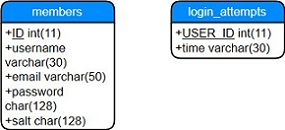
\includegraphics{Bilder/Kapitel4/db_login.jpg}
		\caption[Schematische Darstellung des Datenbankentwurfs des Logins]{Schematische Darstellung des Datenbankentwurfs des Logins}
		\label{fig:Datenbankentwurf_login}
	\end{center}
\end{figure}
Die Datenbank wurde um die Tabellen "'members"' und "'login-attemps"' erweitert. Die Datenbanktabelle "'members"' enthält die selbsterklärenden Attribute "'ID"',"'username"',"'email"',"'password"' und "'salt"'. Die Tabelle "'login-attemps"' besitzt die Attribute "'USER\_ID"' und "'time"'. 

Die genaue Funktionalität des Logins wird nachfolgend in \fullref{login} erläutert.
%Genauere Erklärung durch Harm?
Die Datenbank aus \fullref{sub:Datenbank} wurde wie folgt erweitert:
\begin{figure}[htp]
	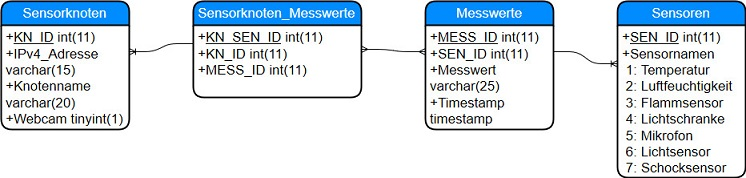
\includegraphics[width=\textwidth]{Bilder/Kapitel4/Datenbankentwurf2.jpg}
	\caption[Schematische Darstellung des erweiterten Datenbankentwurfs]{Schematische Darstellung des erweiterten Datenbankentwurfs}
	\label{fig:Datenbankentwurf_erweiterung}
\end{figure}
Die Datenbanktabelle "'Sensorknoten"' wurde durch das Attribut "'Webcam"' erweitert. Das Attribut "'Webcam"' soll als Flag dienen und durch ihren Zustand (0 oder 1) anzeigen, ob eine Kamera angeschlossen ist. Dies war notwendig, da es keine Möglichkeit gibt, auszulesen ob eine Webkamera installiert ist. Das Attribut "'Webcam"' kann über die Homepage gesetzt werden.

%Erläutern
\subsection{Empfangen der Sensordaten}
Die Scriptsprache Python muss mit folgenden Bibliotheken erweitert werden, damit eine Socketschnittstelle erstellt werden kann und die Sensordaten, aus dem \fullref{Sensorknoten:JSON}, empfangen werden können.
\begin{lstlisting}[caption=Einbinden der Bibliotheken für die Schnittstelle,frame=single,numbers=left,language=Python]
import socket
import json
\end{lstlisting}
Die Bibliotheken socket und json werden eingebunden. Die Bibliothek socket ist dafür zuständig, die Funktionalität der Socketschnittstelle bereitzustellen. Die Bibliothek json ist in diesem Fall nur für die Verarbeitung der Daten zuständig.

Nachfolgend kommt die Bereitstellung der Socketschnittstelle:
% Referenz Methode:senden
\begin{lstlisting}[caption=Bereitstellen der Socketschnittstelle,frame=single,numbers=left,language=Python,showstringspaces=false]
s = socket.socket()
host = '192.168.178.1'
port = 12345
s.bind((host, port))
s.listen(5)
msg = 'Thank you for connecting'
\end{lstlisting}
Mit dem Befehl "'socket.socket()"' wird eine neue Socket-Instanz erzeugt und in der Variable "'s"' gespeichert. Danach wird die IP-Adresse der Zentraleinheit in der Variable "'host"' und ein beliebiger Port der Zentraleinheit in die Variable "'port"' gespeichert. Durch den Aufruf "'s.bind((host, port))"' wird die zuvor gespeicherte IP-Adresse und der Port der Zentraleinheit, an den Socket gebunden. D.h. die Socketschnittstelle der Zentraleinheit ist klientseitig unter der zuvor festgelegten IP-Adresse und Port erreichbar. Mit dem Befehl "'s.listen(5)"' wird die Zentraleinheit in den passiven Modus geschaltet und "'hört"' ob Verbindungsanfragen ankommen. Der übergebene Parameter, in diesem Fall "'5"', bestimmt wie viele Verbindungsversuche gepuffert werden. Bei einer erfolgreichen Verbindung wird die Nachricht in Zeile sechs an den Klienten geschickt.

Im nächsten Codeabschnitt wird beschrieben, wie die Schnittstelle eine Verbindung annimmt und wie die empfangenen Daten gespeichert werden.
\begin{lstlisting}[caption=Speichern der empfangenen Daten,frame=single,numbers=left,language=Python,showstringspaces=false]
while True:
	c, addr = s.accept()
	print('Got connection from ', addr)
	data = json.loads(c.recv(4096).encode('utf-8'))
	Name = str(data["Name"])
	SEN_ID = str(data["SEN_ID"])
	Wert = str(data["Messwert"])
	adresse = str(addr[0])
\end{lstlisting}\label{Daten}
In einer Endlosschleife wartet der Socket mit dem Befehl "'s.accept()"' auf eingehende Verbindungsanfragen. Wenn Verbindungsanfragen eingehen, speichert er im ersten Tupel die empfangenen Daten und im zweiten Tupel Informationen des Absenders. Danach wird ausgeben das eine Verbindung mit der IP-Adresse des Absenders besteht. Der Befehl "'json.loads(c.recv(4096).encode('utf-8'))"' ist für mehrere Dinge zuständig. Der Befehlsteil "'.encode('utf-8')"' gibt vor, dass das empfangene Paket UTF-8-Kodiert sein soll, der Befehlsteil "'c.recv(4096)"' gibt die Paketlänge vor, die in diesem Fall maximal 4096 Bit groß sein darf. Der Befehl "'json.loads"' erzeugt aus den empfangenen Daten ein JSON-Objekt, welches für die weitere Verarbeitung des Paketinhaltes notwendig ist. Das Erzeugen einen JSON-Objekts ist nur möglich, da im \fullref{Sensorknoten:JSON} das Paket als JSON-Objekt gepackt wird. Das erzeugte JSON-Objekt wird in der Variable "'data"' gespeichert. 

Nachfolgend werden die übertragenen Daten herausgefiltert und in die jeweiligen Variablen gespeichert, diese Daten werden für die Befüllung der Datenbank benötigt.

\subsection{Befüllen der Datenbank}
Damit mit Python eine Datenbank befüllt werden kann, muss zuerst eine Bibliothek eingebunden werden.
\begin{lstlisting}[caption=Einbinden der Bibliothek für die Datenbank,frame=single,numbers=left,language=Python]
import MySQLdb as mdb
\end{lstlisting}
Die Bibliotheken MySQLdb wird eingebunden und mdb wird als Alias festgelegt.

Danach muss der Datenbankkonnektor implementiert werden. Nachfolgenden der Quellcode für den Datenbankkonnektor:
\begin{lstlisting}[caption=Datenbankkonnekor,frame=single,numbers=left,language=Python,showstringspaces=false]
try:
	con = mdb.connect('localhost', 'root', 'Piroot',
	'Sicherheitssystem')
	print("SQL-Connection successful")
except _mysql.Error, e:
	print("SQL-Connection failed. Error %d:
	%s" % (e.args[0], e.args[1]))
\end{lstlisting}
Der Datenbankkonnektor ist in zwei Blöcke unterteilt, dem try Block und dem except "'\_mysql.Error"', e Block.

Im try Block wird über die Funktion mdb.connect eine Verbindung hergestellt und in der Variable "'con"' \label{con} gespeichert. Die in den Klammern stehenden Variablen sind von links nach rechts der Hostname, der Benutzername, das Passwort und den Namen der Datenbank, welche angesprochen werden soll. Wenn die Verbindung fehlerfrei hergestellt wurde, wird über die print Funktion die Meldung "'SQL-Connection successful"' ausgegeben.

Im zweiten Block, dem except "'\_mysql.Error"', e Block wird der Fehlerfall abgedeckt. Sollte die Funktion mdb.connect keine erfolgreiche Verbindung herstellen, gibt die print Funktion die Meldung "'SQL-Connection failed. Error \%d:\%s"' aus. An die Stelle des Platzhalters \%d wird der Fehlercode und an den Platzhalter \%s die Fehlermeldung, die zurückgegeben wird, geschrieben, welche die Datenbank liefert.

Im nächsten Abschnitt ist der komplette Quellcode für die Befüllung der Datenbank zu sehen:
\begin{lstlisting}[caption=Befüllung der Datenbank,frame=single,numbers=left,language=Python,showstringspaces=false]
with con:
	cur = con.cursor()
	row_count = cur.execute("SELECT KN_ID FROM Sensorknoten
	WHERE Knotennamen = %s", (Name,))
	# Wenn ein Datenbankeintrag gefunden wird,
	wird die IPv4-Adresse erneuert
	if row_count == 1:
		KN_ID = cur.fetchone()
		cur.execute("""UPDATE Sensorknoten SET
		IPv4_Adresse = %s WHERE
		Knotennamen = %s""", (adresse, Name))
		cur.execute("""INSERT INTO Messwerte 
		(SEN_ID, Messwert) VALUES(%s, %s)""",
		(SEN_ID, Wert))
		# Die zuletzt erstellte ID wird übergeben
		MessID = cur.lastrowid
		cur.execute("""INSERT INTO 
		Sensorknoten_Messwerte (KN_ID, MESS_ID)
		VALUES(%s, %s)""", (KN_ID, MessID))
		# Wenn kein Datenbankeintrag gefunden wird,
		wird ein neuer Datenbankeintrag erstellt
	elif row_count == 0:
		cur.execute("""INSERT INTO Sensorknoten
		(Knotennamen, IPv4_Adresse) VALUES
		(%s, %s)""", (Name, adresse))
		# Die zuletzt erstellte ID wird übergeben
		KN_ID = cur.lastrowid
		cur.execute("""INSERT INTO Messwerte
		(SEN_ID, Messwert)VALUES(%s, %s)""",
		(SEN_ID, Wert))
		# Die zuletzt erstellte ID wird übergeben
		MessID = cur.lastrowid
		cur.execute("""INSERT INTO 
		Sensorknoten_Messwerte(KN_ID, MESS_ID)
		VALUES(%s, %s)""", (KN_ID, MessID))
con.close()
\end{lstlisting}
Der große Block, beginnend mit "'with con"' und endend mit "'con.close()"', beinhaltet die Befüllung der Datenbank. "'with con"' bedeutet, dass der nachfolgende Quellcode mit dem Konnektor aus Kapitel \fullref{con} durchgeführt wird und das "'close.con()"', dass die Verbindung getrennt wird. Im ersten Abschnitt wird mit dem Befehl "'con.cursor()"' ein Cursor-Objekt in der Variable "'cur"' gespeichert. Dieses Cursor-Objekt wird dazu benötigt, um die Datensätze in der Datenbank zu durchlaufen. Mit dem "'cur.execute"' Befehl werden die in der Select-Anweisung festgelegten Datensätze durchsucht und in der Variable "'row\_count"' gespeichert. Die Variable "'row\_count"' dient zur Auswertung, ob ein Datensatz vorhanden ist oder nicht.
 
Ist ein Datensatz vorhanden, springt das Programm in den nachfolgenden if Block.
\begin{lstlisting}[caption=If-Anweisung des Befüllen der Datenbank,frame=single,numbers=left,language=Python,showstringspaces=false]
if row_count == 1:
	KN_ID = cur.fetchone()
	cur.execute("""UPDATE Sensorknoten SET
	IPv4_Adresse = %s WHERE
	Knotennamen = %s""", (adresse, Name))
	cur.execute("""INSERT INTO Messwerte 
	(SEN_ID, Messwert) VALUES(%s, %s)""",
	(SEN_ID, Wert))
	# Die zuletzt erstellte ID wird übergeben
	MessID = cur.lastrowid
	cur.execute("""INSERT INTO 
	Sensorknoten_Messwerte (KN_ID, MESS_ID)
	VALUES(%s, %s)""", (KN_ID, MessID))
\end{lstlisting}\label{If-Anweisung}
 In der If-Anweisung wird überprüft, ob ein Datensatz vorhanden ist. In diesem Block wird zuerst die zuvor selektierete Knotenid mit dem Befehl "'cur.fetchone()"' geholt und in die Variable "'KN\_ID gespeichert"'. Danach wird mit den Daten aus Kapitel \fullref{Daten} der Datenbankeintrag mit dem SQL-Befehl "'UPDATE"' erneuert. Mit dem SQL-Befehl "'INSERT"' wird ein neuer Datensatz in der Datenbanktabelle Messwerte erzeugt. Die ID des zuletzt erstellten Datenbankeintrags wird mit dem Befehl "'cur.lastrowid"' in die Variable "'MessID"' gespeichert. Diese "'MessID"' wird benötigt, damit die Verknüpfung der Datenbanktabellen mit dem nächsten Befehl stattfinden kann. Der letzte "'INSERT"'-Befehl verknüpft die Datenbanken, was wichtig für die spätere Suche nach den richtigen Werten für die Anzeige auf der Webseite ist.
 
 Wenn kein Datensatz gefunden wurde, springt das Programm in die Elseif-Anweisung. 
\begin{lstlisting}[caption=Ifelse-Anweisung des Befüllen der Datenbank,frame=single,numbers=left,language=Python,showstringspaces=false]
	# Wenn kein Datenbankeintrag gefunden wird,
	wird ein neuer Datenbankeintrag erstellt
elif row_count == 0:
	cur.execute("""INSERT INTO Sensorknoten
	(Knotennamen, IPv4_Adresse) VALUES
	(%s, %s)""", (Name, adresse))
	# Die zuletzt erstellte ID wird übergeben
	KN_ID = cur.lastrowid
	cur.execute("""INSERT INTO Messwerte
	(SEN_ID, Messwert)VALUES(%s, %s)""",
	(SEN_ID, Wert))
	# Die zuletzt erstellte ID wird übergeben
	MessID = cur.lastrowid
	cur.execute("""INSERT INTO 
	Sensorknoten_Messwerte(KN_ID, MESS_ID)
	VALUES(%s, %s)""", (KN_ID, MessID))
\end{lstlisting}
 Diese Elseif-Anweisung - in Python "'elif"' genannt - funktioniert ähnlich wie die zuvor vorgestellte If-Anweisung aus Unterabschnitt \fullref{If-Anweisung}, sie unterscheidet sich ausschließich in den ersten paar Zeilen. Anstatt wie zuvor, den mit Hilfe des Knotenamens selektierte Datensatz zu erneuern, wird hier ein neuer Datensatz mit den Daten aus Unterabschnitt \fullref{Daten} erstellt. Die "'Knotenid"' des zuvor erstellten Datensatz wird mit dem Befehl "'cur.lastrowid"' in die Variable "'KN\_ID"' für einen späteren SQL-Befehl gespeichert. Mit dem "'INSERT"' Befehl wird ein neuer Datensatz erstellt, dieser enthält Werte aus dem Unterabschnitt \fullref{Daten}. Auch hier wird wieder die ID, in diesem Fall die MessID"', des zuvor erstellten Datensatzes in die Variable "'MessID"' gespeichert. Die letzte INSERT-Anweisung, verknüpft die Datenbanken mit Hilfe der zuvor gespeicherten ID's.
 %Hacken
\subsection{Problematik Zeitsynchronisierung}\label{Zeitsynchronisierung}
Problematisch bei den Raspberry Pis ist die Zeitsynchronisierung. Die Zeit wird nur synchronisiert und somit aktuell gehalten, wenn der Raspberry Pi mit einem Netzwerk mit funktionierender Internetverbindung verbunden ist. In der Datenbank auf der Zentraleinheit werden Messwerte mit einem Zeitstempel gespeichert. Problematisch ist hierbei, dass ein täglicher Cronjob Messwerte löscht, die älter als eine Woche sind. Um die Problematik mit der Zeitsynchronisierung und damit verbunden Problemen zu lösen, musste eine schnelle und zuverlässige Lösung gefunden werden. Die in \fullref{Sensoren_Planung} vorgestellte Erweiterungsplatine RPi-Explorer 700 von Joy-IT beinhaltet einen internen Zeitgeber. Dieser Zeitgeber, kann die Uhrzeit des Raspberry Pi auf dem aktuellen Stand halten. Dazu muss auf der RPi-Explorer 700 eine Batterie montiert werden und die Funktionalität auf der Zentraleinheit aktiviert werden. Dies geschieht mit folgenden Befehlen auf der Zentraleinheit:
%TODO: Befehle aus Pi auslesen
\begin{lstlisting}[caption=Aktivieren des I2C Bus,frame=single,numbers=left,language=bash,showstringspaces=false]
sudo raspi-config
\end{lstlisting}
Zuerst muss in den Raspberry Pi Einstellungen unter "'raspi-config"' im Menü "'Advanced"' der I2C Bus aktiviert werden.

Danach muss Software zur Konfiguration installiert werden:
\begin{lstlisting}[caption=Installation für die Konfiguration,frame=single,numbers=left,language=bash,showstringspaces=false]
sudo apt-get install python-smbus i2c-tools
\end{lstlisting}
Mit diesem Befehl werden die Pakete "'python-smbus"' und "'i2c-tools"' auf dem Raspberry Pi installiert.

Nachfolgend wir getestet werden, welche Module am I2C-Bus aktiviert sind:
\begin{lstlisting}[caption=I2C-Bus,frame=single,numbers=left,language=bash,showstringspaces=false]
sudo i2cdetect -y 1
\end{lstlisting}
An Position 68 die Zahl 68. Die Zahl 68 ist die Adresse, an welche das Modul geschrieben werden muss.

Nun muss festgestellt werden, welcher RTC Chip verwendet wird, in diesem Fall das Modul ds3231. Dieses Modul muss in die Bootconfig eingefügt werden. Folgender Befehl führt in die Bootconfig:
\begin{lstlisting}[caption=Bootconfig,frame=single,numbers=left,language=bash,showstringspaces=false]
sudo nano /boot/config.txt
\end{lstlisting}
Mit diesem Befehl kann in die Bootconfig geschrieben werden.

An die letzte Zeile muss das zuvor verwendete Modul eingetragen werden:
\begin{lstlisting}[caption=Eintrag Bootconfig,frame=single,numbers=left,language=bash,showstringspaces=false]
dtoverlay=i2c-rtc,ds3231
\end{lstlisting}

Nun muss der Raspberry Pi mit dem Befehl neu gestartet werden: 
\begin{lstlisting}[caption=Neustart Raspberry Pi,frame=single,numbers=left,language=bash,showstringspaces=false]
sudo reboot now
\end{lstlisting}
Danach wird mit folgenden Befehl kontrolliert, ob das neue Modul aktiv ist:
\begin{lstlisting}[caption=I2C-Bus Kontrolle,frame=single,numbers=left,language=bash,showstringspaces=false]
sudo i2cdetect -y 1
\end{lstlisting}
An der Position 68 steht nun keine 68 mehr, sondern UU. D.h. Das neue Modul ist aktiv.

Der alte Zeitgeber muss entfernt werden:
\begin{lstlisting}[caption=Entfernen des Zeitgebers,frame=single,numbers=left,language=bash,showstringspaces=false]
sudo apt-get -y remove fake-hwclock
sudo update-rc.d -f fake-hwclock remove
\end{lstlisting}
Mit diesen beiden Befehlen wird der alte Zeitgeber entfernt.

Anschließend muss das Skript des alten Zeitgebers auskommentiert werden. Diese befindet sich in folgender Datei:
\begin{lstlisting}[caption=Zeitgeber Skript,frame=single,numbers=left,language=bash,showstringspaces=false]
sudo nano /lib/udev/hwclock-set
\end{lstlisting}
Hier müssen die Zeilen:
\begin{lstlisting}[caption=Auskommentieren in Zeitgeber Skript,frame=single,numbers=left,language=bash,showstringspaces=false]
#if [ -e /run/systemd/system ] ; then
# exit 0
#fi
\end{lstlisting}
Mit dem nächsten Befehl kann überprüft werden ob der alte Zeitgeber deaktiviert wurde:
\begin{lstlisting}[caption=Überprüfung des alten Zeitgebers,frame=single,numbers=left,language=bash,showstringspaces=false]
hwclock -D -r
\end{lstlisting}
Ist der alte Zeitgeber deaktiviert, kann das neue Zeitgebermodul synchronisiert werden.

Hierzu muss der Raspberry Pi an ein internetfähiges Netzwerk angeschlossen werden. Der Raspberry Pi holt sich automatisch die aktuelle Zeit aus dem Internet.

Die synchronisierte Zeit muss auf das neue Zeitgebermodul geschrieben werden:
\begin{lstlisting}[caption=Schreiben der Zeit auf das Zeitgebermodul,frame=single,numbers=left,language=bash,showstringspaces=false]
sudo hwclock -w
\end{lstlisting}
Nun ist die synchronisierte Zeit aus dem Internet auf das neue Zeitgebermodul geschrieben. Der Raspberry Pi kann vom Internet entfernt werden.

Mit dem nachfolgenden Befehl kann überprüft werden, ob die Zeit des neuen Zeitgebers aktuell ist:
\begin{lstlisting}[caption=Lesen der Zeit auf das Zeitgebermodul,frame=single,numbers=left,language=bash,showstringspaces=false]
sudo hwclock -r
\end{lstlisting}
Die aktuelle Zeit des Zeitgebers wird ausgegeben. Die Zeit auf dem Raspberry Pi wird nun von dem neuen Zeitgeber ohne Internetverbindung aktuell gehalten.
\section{Webseite} \label{Webseite}
%Harm
\subsection{Login und Logout}\label{login}

Der Login, die Registrierung und der Logout ist nach der Anleitung von
wikiHow (\cite{PHP-Login:online}) erstellt und entsprechend angepasst worden. 
\\
Der Login, der in \fullref{pic:login} zu sehen ist, besteht aus mehreren Dateien, deren Funktion in der Tabelle
(\nameref{tab:Login-Dateien}) aufgezählt ist.

\begin{figure} [htb]
\begin{centering}
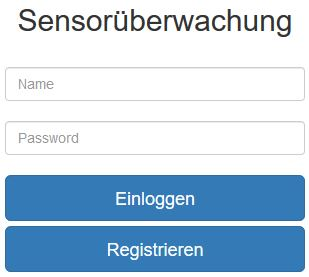
\includegraphics{Bilder/Kapitel4/login.jpg}
\caption[Ansicht des Logins]{Ansicht des Logins}
\label{pic:login}
\end{centering}
\end{figure}

\begin{table}
\caption{PHP-Login-Dateien und Funktion}
\label{tab:Login-Dateien}
\begin{tabular}{p{0.5\textwidth} p{0.45\textwidth}}
\textbf{Datei} 				& \textbf{Erklärung} \\
Login.php 						& Die Loginseite - Gleichzeitig auch die Startseite bei Aufruf der Server-IP\\
Register.php 					& Die Registrierungsseite \\
Register\_success.php & Die Seite, die nach einer erfolgreichen Registrierung angezeigt wird \\
Logout.php 						& Die Seite, die nach einem erfolgreichen Logout angezeigt wird \\
psl\_config.php 			& Festlegung von Variablen, die mehrfach verwendet werden \\
db-connect.php 				& Datenbank-Connector \\
functions.php 				& Relevante Funktionen, die benötigt werden \\
process\_login.php 		& Code der die Logindaten der Loginseite überprüft und danach auf die Übersichtsseite weiterleitet \\
register\_inc.php 				& Code der abläuft, wenn sich ein User neu registriert \\
forms.js 							& Javascriptdatei, für das Hashen und Überprüfen der Passwörter \\
sha512.js 						& JavaScript-Implementierung der Hashfunktion SHA-512 (\cite{sha512js:online})\\
style.css 						& CSS-Datei für zentrale Designeinstellungen \\
 \end{tabular}
\end{table}

In der Datei functions.php sind zentrale Funktionen gesammelt, die nachfolgend
beschrieben werden:

%Hacken
\subsubsection{sec\_session\_start}
%TODO: Session-ID und Cookie erklähren - Erledigt?
Diese Funktion vergibt eine Session-ID und legt fest, dass Cookies verwendet werden. Die Session-ID ermöglicht es Anfragen eines Clients zuordnen zu können und Antworten oder Aktualisierungen an diesen zu senden. Die Session-ID wird vom Server generiert und per Cookie an den Client übertragen. Der Client speichert das Cookie ab und sendet bei jeder Anfrage das Cookie (mit der Session-ID) an den Server. Wird keine oder eine falsche Session-ID übertragen erhält der Benutzer, die Meldung, dass er sich zuerst am System anmelden muss. Durch den Anmelde-Vorgang wird dem Client eine neue Session-ID zugewiesen.

\subsubsection{login}
Diese Funktion steuert alle notwendigen Abläufe, die den Login betreffend.\\
Aufgerufen wird die Funktion mit den Parametern Username, Passwort und der Datenbankverbindung. Die Parameter Username und Passwort werden aus POST-Werten der Loginseite übergeben während die Datenbankverbindung in der Datei db-connect.php definiert ist. Durch ein Prepared-Statement werden die benötigten Werte aus der Datenbank abgerufen. Danach wird verglichen ob der übergebene Username in der Datenbank hinterlegt ist. Existiert der Benutzer, wird zuerst durch die Funktion 'checkbrute' überprüft, ob der Benutzer momentan gesperrt ist. Ist der Benutzer nicht gesperrt, wird das Passwort überprüft und der Anwender wird auf die Seite 'Übersicht' weitergeleitet. Ist das Passwort nicht korrekt, wird der fehlgeschlagene Loginversuch in der Datenbank vermerkt und der Benutzer erhält eine Meldung wie in \fullref{computersaysno}, dass der Anmeldeversuch fehlgeschlagen ist.

\begin{figure} [htb]
\begin{centering}
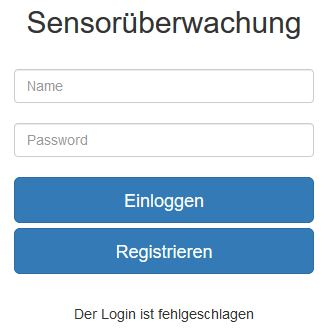
\includegraphics{Bilder/Kapitel4/login_fehlgeschlagen.jpg}
\caption[Meldung bei einer falschen Benutzer/Passwort Kombination]{Meldung bei einer falschen Benutzer und Passwort Kombination}
\label{computersaysno}
\end{centering}
\end{figure}

%CHECK
\subsubsection{checkbrute}
Die Funktion "`checkbrute()"' prüft, ob  ein Angreifer möglicherweise versucht eine Brute-Force-Attacke durchzuführen. Eine Brute-Force-Attacke ist das systematische Ausprobieren von Kennwörtern. Ein Kennwort kann mittels Brute-Force-Attacke immer irgendwann herausgefunden werden. Die einzige Schutzmöglichkeit besteht darin, den Aufwand unermesslich groß zu machen. Ein handelsüblicher PC kann mittlerweile mehrere Millionen von Passwörtern pro Sekunde ausprobieren. Dies führt dazu, dass ein einfaches (kurzes) Passwort sehr schnell geknackt werden kann. Ein Passwort, dass nur aus Kleinbuchstaben besteht und ein Zeichen lang ist, hat somit 26 verschiedene Möglichkeiten. Wird die Länge auf 2 erhöht, gibt es bereits $26^2$ verschiedene Möglichkeiten. Ein aktuelles Passwort sollte immer mindestens 8 Zeichen lang sein und mindestens einen Kleinbuchstaben, einen Großbuchstaben, eine Zahl und ein Sonderzeichen enthalten. Daraus ergibt sich $94^8$ was 6.095.689.385.410.816 verschiedenen Möglichkeiten entspricht. Durch eine "`Bremse"' kann die Dauer bis alle potentiellen Passwörter ausprobiert wurden weiter erhöht werden. Eine solche "`Bremse"' ist beispielsweise das von der Funktion "`checkbrute()"' eingesetzte blockieren von weiteren Einloggversuchen nach 5 fehlgeschlagenen Eingaben.

Die Funktion "`checkbrute()"' prüft, ob in den letzten zwei Stunden mehr als 5 fehlgeschlagene Einloggversuche protokolliert wurden und sperrt den Benutzer. Der Benutzer muss erst über die Datenbank wieder freigeschaltet werden, bevor ein erneutes Einloggen wieder möglich ist.

\subsubsection{login\_check}
Diese Funktion prüft, ob ein Anwender eingeloggt ist und setzt den entsprechenden
Parameter, der entscheidet, was der Anwender auf der Website sieht. Ist der Anwender korrekt eingeloggt sieht er die korrekte Webseite. Für den Fall, dass der Anwender nicht eingeloggt ist sieht er wie in \fullref{notloggedin} die Information, dass er sich bitte einloggen soll.

\begin{figure} [htb]
\begin{centering}
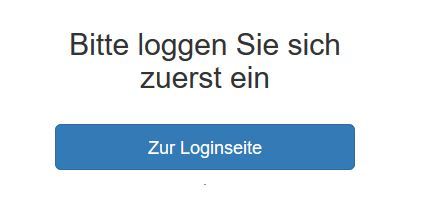
\includegraphics{Bilder/Kapitel4/notloggedin.jpg}
\caption[Meldung wenn der Anwender nicht eingeloggt ist]{Meldung wenn der Anwender nicht eingeloggt ist}
\label{notloggedin}
\end{centering}
\end{figure}


\subsubsection{esc\_url}
%TODO: prüfen
Auf der Registrierungsseite finden Benutzereingabe statt, die in die Datenbank geschrieben werden. Um Cross-Site-Scripting zu verhindern, wird diese Funktion dafür verwendet um die Benutzereingaben zu "`bereinigen"'. Die Bereinigung findet über einen Regulären Ausdruck statt, der alle sinnvollen Zeichen ausschließt und durch "`nichts"' ersetzt. Als Folge daraus bleibt das "`Action"'-Attribut, des Eingabeformulars leer. Dies ist nicht weiter problematisch, da die Registrierung über die anderen Skripte abgewickelt wird.

\subsubsection{forms.js}
In der Datei forms.js sind zwei Funktionen enthalten. Die Funktion "`formhash"' wird beim regulären Login verwendet und die Funktion "`regformhash"' wird bei der Registrierung verwendet. \\
Mit der Funktion "`formhash"' wird das Passwort, dass auf der Login-Seite im Passwortfeld steht mithilfe des Hashalgorithmusses gehasht und in ein nicht sichtbares Feld eingefügt. Die Passwortüberprüfung auf der Serverseite verwendet danach nur noch das gehashte Passwort für den Vergleich mit der Datenbank.\\
Die Funktion "`regformhash"' ist etwas aufwendiger, da sie bei der Registrierung verwendet wird. Im ersten Schritt wird geprüft ob in jedem Feld eine Eingabe vorhanden ist. Ist dies nicht der Fall wird dem Anwender mitgeteilt, dass er alle Felder ausfüllen muss. Im zweiten Schritt werden die verschiedenen Eingaben überprüft ob sie die Bedingungen erfüllen, die festgelegt wurden. Im dritten Schritt wird überprüft ob die Passwörter gleich sind. Anschließend wird wie bei der Funktion "`formhash"' auch ein nicht sichtbares Feld eingefügt, in dem das gehashte Passwort gespeichert wird. Die Klartextpasswörter, die in den Eingabefeldern stehen, werden gelöscht damit sie nicht übertragen werden. Im letzten Schritt wird das Formular abgeschickt.

\subsubsection{Logout}
Beim Logout ist nur die Datei logout.php beteiligt. Die Datei wird nach dem Klick auf Logout aufgerufen und löscht die Session-ID, das aktuelle Cookie und beendet die Sitzung. Als letztes wird auf die Login-Seite weitergeleitet.

\begin{lstlisting}[caption=Inhalt der logout.php,frame=single,numbers=left,language=PHP]
include_once 'functions.php';
sec_session_start();
// Setze alle Session-Werte zurück
$_SESSION = array();
// hole Session-Parameter
$params = session_get_cookie_params();
// Lösche das aktuelle Cookie.
setcookie(session_name(),
    '', time() - 42000,
    $params["path"],
    $params["domain"],
    $params["secure"],
    $params["httponly"]);
// Vernichte die Session
session_destroy();
header('Location: ../../Login.php');
\end{lstlisting}

%Jan
\subsection{Übersicht}\label{Uebersicht}
Die Übersichtsseite zeigt einen Übersicht über die angeschlossenen Sensorknoten und die Werte der einzelnen Sensoren der Sensorknoten an. Auf der Webseite werden nur die Sensorknoten mit ihren Sensoren angezeigt die sich tatsächlich im Netz befinden. Dafür zuständig ist die Datei sensordaten.php. Die Datei sensordaten.php ladet die Werte aus der Datenbank und erstellt daraus dynamisch eine Anzeigetabelle der Sensorknoten und den zugehörigen Sensoren. Die Anzeigetabelle zeigt alle Sensoren an, die an den jeweiligen Sensorknoten angeschlossen sind. Falls Sensoren nicht angeschlossen sind, wird das in der Tabelle angezeigt. Zusätzlich wird unter jede Tabelle ein Symbol mit der Verlinkung zu den Statistiken(siehe \fullref{Statistik}) und der Webkameras(siehe \fullref{Webkamera}) angezeigt, dies hat den Zweck zum schnelleren Wechsel auf die jeweilige Seite. Des weiteren wird die Seite alle fünf Sekunden automatisch nachgeladen, dies geschieht über die uebersichtscript.js und sorgt dafür, dass die angezeigten Daten aktuell sind ohne die Seite manuell zu aktualisiert werden.

Die Besonderheit der Übersichtsseite ist die Datenbankabfragen, sie setzt sich aus mehreren Befehlen zusammen. Die Abfrage findet in der Datei sensordaten.php statt und kann wie folgt Visualisiert werden:
\begin{figure}[htp]
	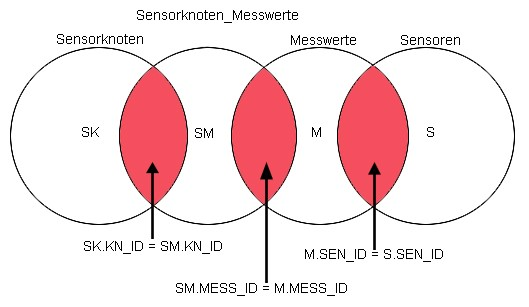
\includegraphics[width=\textwidth]{Bilder/Kapitel4/uebersichtjoin.jpg}
	\caption[Mengendarstellung der Übersichtsseite]{Selbsterstelle Darstellung des Join Befehls über die Tabellen Sensorknoten, Sensorknoten\_Messwerte, Messwerte und Sensoren}
	\label{fig:Kapitel4/uebersichtjoin.jpg}
\end{figure}
Die Datenbankabfrage besteht aus vier einzelnen Tabellen, diese müssen zu einer zusammengeführt und gefiltert werden. Die Tabellen sind "'Sensorknoten"', "'Sensorknoten\_Messwerte"', "'Messwerte"' und "'Sensoren"'. Die Tabellen werden mit, wie in der Darstellung zusehen, mit ihren Schlüsseln mit einander Verknüpft. Hierzu werden die Primärschlüssel und die Fremdschlüssel der jeweiligen Tabellen mit einander abgeglichen. Durch diesen Vorgang wird eine "'virtuelle Tabelle"' erstellt. Ziel dieser Verknüpfung ist es, die Messwerte der jeweiligen Sensoren eines Sensorknoten zu filtern und auszugeben.

% Erklärung Alex
%1. Selection von allem
%2. Aufbau einer virtuellen Tabelle (Mysql-Lösung, da es keine echten virtuellen Tabellen gibt (with ...))
%3. From Sensorknoten SK -> "SK" ist alias für die Tabelle Sensorknoten, erste Tabelle benötigt das wort "as" nicht
%4. Hilfstabelle Sensorknoten_Messwerte (SM) wird über die ID mit der Sensorknoten (SK) Tabelle verknüpft
%5. Same
%6. Same
%7. Where Klausel Bestimmt mit $Knotennamen den selektierten Knotennamen
%8. Absteigende Sortierung -> Aktuellster wert steht zuerst
%9. Virtue Tabelle ist sortiert und hat den alias sub
%10. Gruppierung -> Dopplungen fallen raus
%11. Sortierung nach Sensor ID
%Bild

%Alex
\newpage
\subsection{Statistik}\label{Statistik}
	Die Messdaten der jeweiligen Sensorknoten können für eine Visualisierung genutzt werden. Da die Daten mit jeweils einem eindeutigen Zeitstempel versehen werden, können diese für einen Graphen mit einer Zeitabhängigkeit genutzt werden. Die notwendigen Daten werden mit Hilfe des Joins der \fullref{fig:Kapitel4/uebersichtjoin.jpg1} zusammengebaut.
	\begin{figure}[htp]
		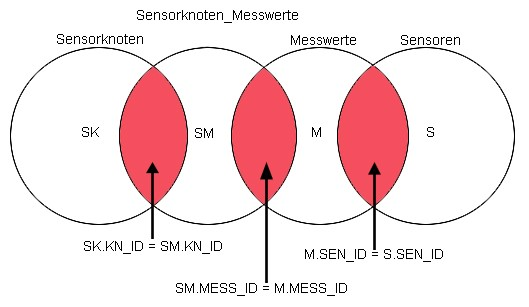
\includegraphics[width=\textwidth]{Bilder/Kapitel4/uebersichtjoin.jpg}
		\caption[Mengendarstellung der Übersichtsseite]{Selbsterstelle Darstellung des Join Befehls über die Tabellen Sensorknoten, Sensorknoten\_Messwerte, Messwerte und Sensoren}
		\label{fig:Kapitel4/uebersichtjoin.jpg1}
	\end{figure}
%TODO Screenshot der Statistik seite einbinden + erklären
	Die Statistikseite ist wie folgt aufgebaut:
	\begin{description}
		\item[1. Sensorknotenauswahl] \hfill \\
			Dieses Dropdownfeld generiert mit Hilfe des folgenden Befehls die Auswahl der Sensorknoten:
\begin{lstlisting}[caption=SQL Selektion der Möglichen Sensorknoten,frame=single,numbers=left,language=SQL]
	SELECT Knotennamen FROM Sensorknoten
\end{lstlisting}
			Ein Sensorknoten wird nur in die Datenbank eingetragen falls er Daten an die Zentaleinheit sendet. Daher reicht dieser Befehl aus, um alle möglichen Sensorknoten auszulesen. Die Rückgabemenge wird mittels dem "'append()"' Befehl an das Dropdownmenü angehängt.
		\item[2. Sensorauwahl] \hfill \\
			In diesem Dropdownfeld werden die jeweils möglichen Sensoren des zuvor ausgewählten Sensorknotens gelistet. Die Menge wird durch das \fullref{Sensorauswahl:Statistik} generiert werden.
			\newpage
\begin{lstlisting}[label={Sensorauswahl:Statistik},caption=Auswahl der Sensoren auf der Statistikseite,frame=single,numbers=left,language=SQL]
Select * FROM(
	SELECT Sensorname FROM Sensorknoten SK
		INNER JOIN Sensorknoten_Messwerte 
			AS SM ON (SK.KN_ID = SM.KN_ID)
		INNER JOIN Messwerte 
			AS M ON (SM.MESS_ID = M.MESS_ID)
		INNER JOIN Sensoren 
			AS S ON (M.SEN_ID = M.MESS_ID)
	WHERE Knotennamen = '".$sensorknoten."'
)AS Stub ORDER BY Sensorname;";
\end{lstlisting}
	Die Join Verkettung über die jeweiligen Primärschlüssel der Tabellen Sensorknoten, der Hilfstabelle Sensorknoten\_Messwerte, Messwerte und Sensoren liefert die angeschlossenen Sensoren an den ausgewählten Sensorknoten. Die \fullref{fig:Kapitel4/uebersichtjoin.jpg1} stellt den Vorgang Listings gleich dar.

	\item[3. Tagesauswahl] \hfill \\
		In diesem Dropdownfeld kann entweder ein möglicher Tag oder die komplette Woche ausgewählt werden. Abhängig von dieser Auswahl wird der Graph entsprechend skaliert. 
	\item[4. Graphische Darstellung] \hfill \\
		Hier werden die ausgewählten Daten durch das Framework "'CanvasJS"' generiert. 
	\item[4. Generierungsbutton] \hfill \\
		Der Button "'Auswahl"' löst beim draufdrücken die Generierung der Darstellung aus.
	\end{description}
Neben dem Aufbau der Seite müssen die Daten aus der Datenbank für die Erstellung der Graphen entsprechend angepasst werden. In diesem Fall gibt es zwei Arten von Messwertdaten  – diskrete und nicht diskrete Daten. Zu den diskreten Messdaten zählen die Temperatur- und Luftfeuchtigkeitsmessungen. Auf der anderen Seite befinden sich die binären Messdaten des Flammensensors, die Geräuschmessung des Mikrofons, die Lichtschranke und der Lichtsensor.\\
Die Messdaten werden beim klicken des "'Auswahl"' Buttons mittels eines \ac{AJAX} Befehls asynchron abgefragt. Daraufhin werden die Daten entweder boolischen oder nummerischen Werten zugeordnet. Im nächsten Schritt werden die Messdaten an das Framework "'canvasJS"' übergeben. Dieses Generiert mit Hilfe der Messdaten, den Zeitraum und der Achsenbeschriftung einen Graphen aus diesen Daten.\\
Bei nummerischen Graphen kann , abhängig von den Messintervallen, der Nutzer in diesen hineinzoomen und genaue Information über die Messwerte erhalten. Der zeitliche Verlauft dient hauptsächlich zur Nachbetrachtung der Messdaten.\\
Aktuelle Informationen der Sensoren können mit Hilfe der Webkamera kontrolliert werden und falls eine Gefahr besteht, kann der Nutzer dementsprechend handeln.
%Alex+Jan
\subsection{Webkamera}\label{Webkamera}
Die Anzeige der Webkamera Seite erfolgt durch die Datei Kamera.php. Funktionserweiterungen über die Dateien kamera.js, kamera.php, kameraadresse.php,  kameraconfig.php und sensorknotenauswahl.php. Hierbei hat jede Datei eine gesonderte Aufgabe und kann bei Bedarf geändert werden ohne das die Funktionalität anderer Dateien beeinträchtigt wird.
\begin{description}
	\item[kamera.js] \hfill \\
	Die Befüllung der Dropdown-Menüs übernimmt die Datei "'kamera.js"'. Diese lädt dynamisch die Daten aus der Datenbank mit Hilfe der anderen Dateien in die Dropdown-Menüs.
	\item[kamera.php] \hfill \\
	In dieser Datei werden die Sensorknoten aus der Datenbank gefiltert, die eine aktivierte Kamera angeschlossen haben.
	\item[sensorknotenauswahl.php] \hfill \\
	Die "'sensorknotenauswahl.php"' selektiert alle Knotennamen der Sensorknoten.
	\item[kameraadresse.php] \hfill \\
	Diese Datei selektiert die Ip-Adresse des jeweiligen Sensorknoten.
	\item[kameraconfig.php] \hfill \\
	Ist dafür zuständig die geänderten Einstellungen in der Datenbank zu speichern.
\end{description}
Auf der Webkamera Seite werden zunächst nur ein Icon für die Einstellungen und ein Dropdown-Menü mit den Sensorknoten die eine aktivierte Kamera haben. Die Sensorknoten mit den aktivierten Kameras können in dem Dropdown-Menü ausgewählt werden. Mit dem "Blablub-Button" kann eine Verbindung zur ausgewählten Kamera hergestellt werden, diese wird nach drücken des Buttons unterhalb der Auswahl angezeigt. In den Einstellungen kann über ein Dropdown-Menü der jeweilige Sensorknoten ausgewählt und über die Radiobuttons die Webkamera aktiviert bzw. deaktiviert werden. In den Dropdown-Menüs werden nur die Sensorknoten angezeigt, die mit der Zentraleinheit verbunden sind. 
%Harm
\subsection{Impressum}

Auf der Seite "`Impressum"' stehen die Namen der drei Autoren, der Titel des Projektes und diese Dokumentation wird zum Download angeboten. Ansonsten ist keine weitere Funktionalität implementiert.
%Alle
\section{Refactoring}
%Alle
\section{Systemtest}
